\documentclass[11pt]{article}

\usepackage[margin=1in]{geometry}
\usepackage{amsmath}
\usepackage{amssymb}
\usepackage{graphicx}
\usepackage[hidelinks]{hyperref}

\newcommand{\softmax}{\operatorname{softmax}}

\title{\textbf{Exercise 04: Rotary Position Embedding (RoPE)}}
\author{}
\date{}

\begin{document}
\maketitle

\begin{center}
\emph{A controlled 2D derivation of how absolute rotations expose relative position in query-key dot products.}
\end{center}

\section*{Setup}

Use positions $p\in\{0,1,2\}$, angle step $\theta=1$ radian, and the same unit query/key vector at every position:
\[
q_p=k_p=\begin{bmatrix}1&0\end{bmatrix}.
\]
The standard rotation matrix is
\[
R(\phi)=
\begin{bmatrix}
\cos\phi&-\sin\phi\\
\sin\phi&\cos\phi
\end{bmatrix}.
\]
With row-vector notation,
\[
q_p^R=q_pR(p\theta)^\top,
\qquad
k_p^R=k_pR(p\theta)^\top.
\]

\section*{1. Without positional rotation}

All base query/key rows are identical, so
\[
QK^\top=
\begin{bmatrix}
1&1&1\\
1&1&1\\
1&1&1
\end{bmatrix}.
\]
After scaling by $\sqrt{d_k}=\sqrt{2}$, every row still contains three equal logits. Therefore
\[
A_{\mathrm{plain}}=
\begin{bmatrix}
\frac13&\frac13&\frac13\\
\frac13&\frac13&\frac13\\
\frac13&\frac13&\frac13
\end{bmatrix}.
\]
With no position-dependent operation, identical content vectors remain indistinguishable to the score function.

\section*{2. Rotate by absolute position}

Because the base vector is $[1,0]$, rotating by angle $p\theta$ gives
\[
q_p^R=k_p^R=
\begin{bmatrix}
\cos(p\theta)&\sin(p\theta)
\end{bmatrix}.
\]
Hence
\[
Q_R=K_R\approx
\begin{bmatrix}
1.0000&0.0000\\
0.5403&0.8415\\
-0.4161&0.9093
\end{bmatrix}.
\]

\begin{figure}[h]
    \centering
    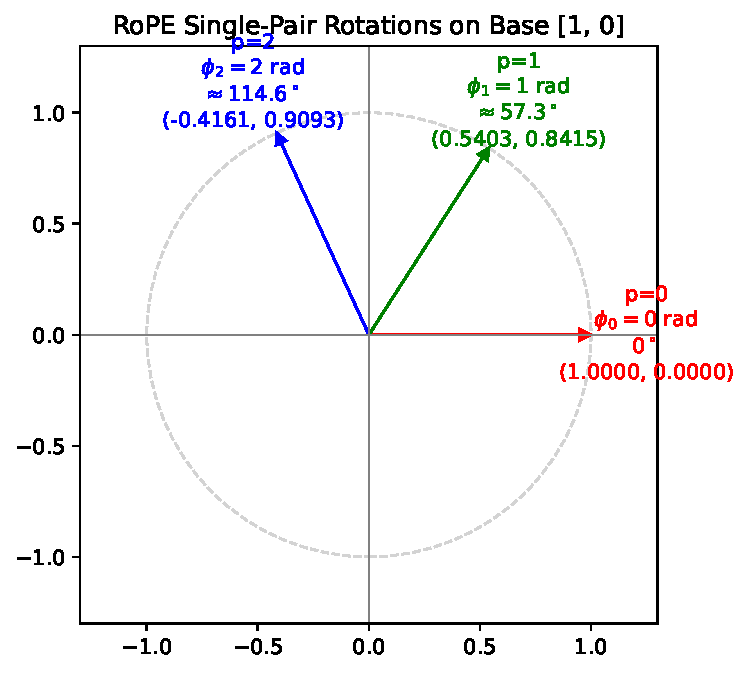
\includegraphics[width=0.58\textwidth]{figures/rope_unit_circle.pdf}
    \caption{The same base vector rotated by the absolute position indices $0$, $1$, and $2$.}
\end{figure}

\section*{3. Compute the RoPE score matrix}

The rotated dot products are
\[
S_{\mathrm{RoPE}}=Q_RK_R^\top
\approx
\begin{bmatrix}
1.0000&0.5403&-0.4161\\
0.5403&1.0000&0.5403\\
-0.4161&0.5403&1.0000
\end{bmatrix}.
\]
Entries with the same relative offset match. For example,
\[
S_{01}=S_{12}\approx0.5403.
\]
The diagonal equals $1$ only because this controlled example uses identical unit query/key vectors. It is not a general property of attention scores.

\section*{4. Derive the relative-position identity}

For query position $m$ and key position $n$,
\[
q_m^R=q_mR(m\theta)^\top,
\qquad
k_n^R=k_nR(n\theta)^\top.
\]
Then
\[
\begin{aligned}
q_m^R(k_n^R)^\top
&=q_mR(m\theta)^\top
\left(k_nR(n\theta)^\top\right)^\top\\
&=q_mR(m\theta)^\top R(n\theta)k_n^\top.
\end{aligned}
\]
Using
\[
R(a)^\top R(b)=R(b-a),
\]
we obtain
\[
\boxed{
q_m^R(k_n^R)^\top
=q_mR((n-m)\theta)k_n^\top
}.
\]
The rotations were chosen using absolute positions $m$ and $n$, but the dot product contains their difference $n-m$.

\begin{figure}[h]
    \centering
    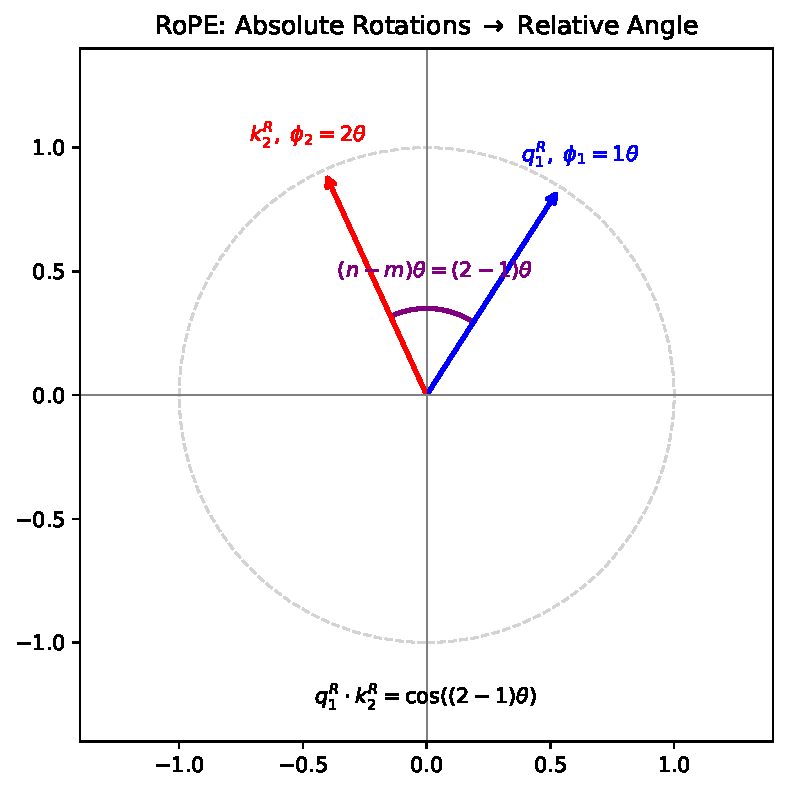
\includegraphics[width=0.58\textwidth]{figures/rope_relative_angle.pdf}
    \caption{The angular difference between absolute rotations is the relative offset signal exposed by the dot product.}
\end{figure}

For this specific base vector $q_m=k_n=[1,0]$,
\[
q_mR((n-m)\theta)k_n^\top
=\cos((n-m)\theta),
\]
so
\[
\boxed{S_{mn}=\cos((n-m)\theta)}.
\]
This cosine-only expression is specific to the controlled unit-vector setup; the boxed matrix identity above is the general 2D statement.

\section*{5. Scale and apply softmax}

Scaling by $\sqrt{2}$ gives
\[
S_{\mathrm{scaled}}
\approx
\begin{bmatrix}
0.7071&0.3821&-0.2943\\
0.3821&0.7071&0.3821\\
-0.2943&0.3821&0.7071
\end{bmatrix}.
\]
Applying row-wise softmax yields
\[
A_{\mathrm{RoPE}}
\approx
\begin{bmatrix}
0.4785&0.3457&0.1758\\
0.2955&0.4090&0.2955\\
0.1758&0.3457&0.4785
\end{bmatrix}.
\]
Unlike the plain uniform attention matrix, the rotated scores distinguish positions even though all base content vectors were identical.

\section*{6. Norm preservation}

Rotation matrices are orthogonal:
\[
R(\phi)^\top R(\phi)=I.
\]
Therefore
\[
\|q_p^R\|_2=\|q_p\|_2,
\qquad
\|k_p^R\|_2=\|k_p\|_2.
\]
RoPE changes orientation, not vector length.

\section*{Final answer}

RoPE uses absolute position indices to choose rotations, but the query-key dot product combines those rotations through
\[
R(m\theta)^\top R(n\theta)=R((n-m)\theta).
\]
That is why relative position appears in the resulting compatibility score.

\section*{Numerical verification}

The companion \texttt{answer\_key.py} verifies the plain and rotated score matrices, the relative-offset equalities, the attention values, and norm preservation. The separate \texttt{generate\_figures.py} script regenerates the two explanatory PDFs in \texttt{figures/}.

\end{document}
